
\documentclass[a4paper]{efr}

\usepackage{verbatim}
\usepackage{graphicx}
%\usepackage{ctable}
%\usepackage{longtable}
%\usepackage{rotating}
%\usepackage{makecell}

%\bibliographystyle{plain}

\def\fboxsep{5pt}
  \newenvironment{myboxenv}[1]
  {
    \begin{flushright}
      \begin{boxedminipage}{0.9\textwidth}
        \textbf{%% \sffamily
          \large #1:}

        \hspace{-5pt}\rule{0.3\textwidth}{0.5pt}
        \begin{center}
          \begin{minipage}{0.95\textwidth}

            \small%% \slshape
         }
          {
          \end{minipage}
        \end{center}
      \end{boxedminipage}
    \end{flushright}
 }

\title{The Enlightenment Foundation Libraries\\
  \normalsize{Prise en main de Edje}}

\EfrMail{aguirre.nicolas@gmail.com}
\author{Nicolas Aguirre}

\begin{document}

\maketitle
\tableofcontents

\section{Avant Propos}

Le but de ce tutoriel est de survoler au travers d'un exemple pratique toutes
les fonctionnalités de Edje.

J'espère qu'il vous permettra également de vous faire comprendre comment Edje
peut vous aider dans le développement de vos interfaces graphiques.

De considérer cette technologie comme l'un des outils les plus puissant des
EFL plutôt que comme votre plus grand cauchemar.

Comment, en séparant la logique et le code d'une part et l'interface d'une
autre, vos interfaces graphiques peuvent gagner en flexibilité.

Comme exemple concret, permettant d'illustrer cette présentation, j'ai choisis
le développement d'un interface (tactile) très simple.
Voici à quoi ressemblera l'interface à la fin de ce tutoriel :

\section{Introduction}

Edje est une des briques de base des EFL. Elle vous permet de décrire une
interface graphique sans écrire une seule ligne de C. Ce qui permet,de facto,
de réaliser une des choses les plus complexes lors du développement d'un
programme avec une interface utilisateur : la séparation de l'interface et du
code. Cette séparation est importante à plus d'un titre. Elle permet d'une part
d'avoir la logique du programme et la gestion des données d'un côté et
l'interface utilisateur de l'autre. Elle permet donc d'avoir deux équipes
distinctes qui travaillent sur le projet, les graphistes, designer, ergonomes et
les développeurs.

Parler de ``Edje'', c'est employer un terme générique pour 3 concepts
différents:
\begin{itemize}
\item Le format de description, le format EDC, pour Edje Data Collection;
\item Le fichier binaire EDJ, résultante compilée de toutes les ressources
décrites dans le fichier EDC;
\item La bibliothèque de fonctions libedje.so, permettant de manipuler les
objets décrits dans le EDC au niveau de Evas.
\end{itemize}

Le schémas ci dessus montre à quel moment ces trois concepts sont utilisés lors
de la création d'une application utilisant Edje :

\begin{figure}
  \begin{center}
    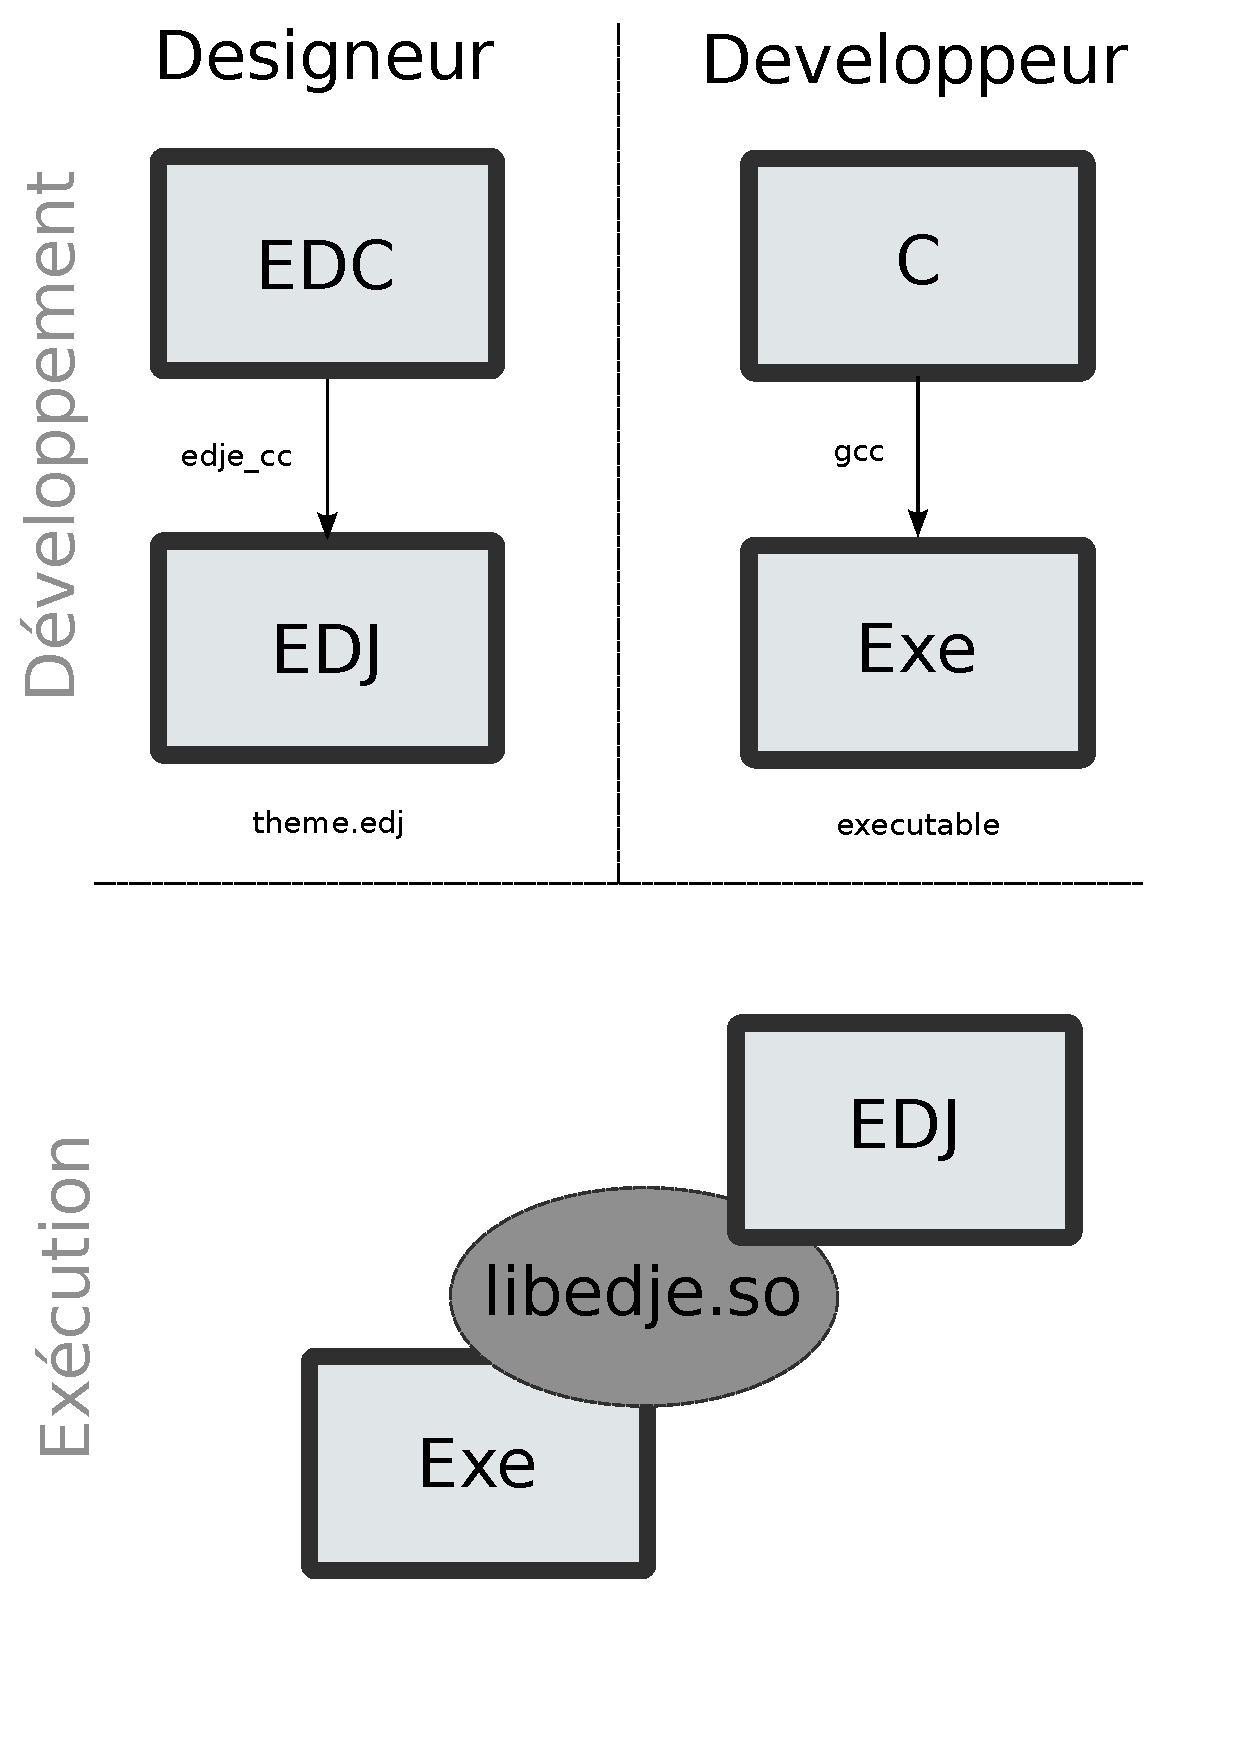
\includegraphics[scale=0.7]{images/workflow.pdf}
  \end{center}
  \caption{Edje Workflow}
\end{figure}

\section{Les Bases}

Dans ce chapitre, nous allons voir les bases du langage de description EDC.

Un fichier EDC (Edje Data Collection) minimal ressemble à ceci : (fichier
tut01/tut01.edc)

\begin{lstlisting}[language=c]
 collections {
   group {
      name: "interface";
      parts {
         /* Rectangle Rouge */
         part {
            name: "Rectangle";
            type: RECT;
            description {
               state: "default" 0.0;
               color: 255 0 0 255;
            }
         }
      }
   }
}
\end{lstlisting}

Nous pouvons voir dans cet exemple le mot clef ``collection'' qui comme son
nom l'indique est un ensemble. Pour un fichier Edje, c'est un ensemble
de ``groupes''.
Dans cet exemple nous avons un seul groupe, nommé ``interface''.
Un groupe est lui-même un ensemble, et représente un objet, qui pourra être
manipulé sur le canvas graphique plus tard dans notre programme ou réutilisé
dans le fichier EDC.
Un Group contient des ``parts'' qui sont les primitives que sait manipuler Evas.
Voici une liste exhaustive des ``parts'' que nous pouvons utiliser :
\begin{itemize}
\item Les rectangles : RECT;
\item Les images : IMAGE;
\item Les textes : TEXT;
\item Les blocs de texte : TEXTBLOCK;
\item Les containers : SWALLOW;
\item Les groupes : GROUP;
\item Les boites : BOX;
\item Les tables : TABLE;
\item Les objets externes : EXTERNAL;
\end{itemize}
Chaque type fera l'objet d'une étude plus approfondie dans la suite de ce
tutoriel.

Dans notre exemple nous décrivons donc un Rectangle rouge, rien de bien
original. Nous allons maintenant compiler ce fichier EDC en un fichier binaire
EDJ.  :

\begin{lstlisting}
edje_cc tut01.edc
\end{lstlisting}

Si la compilation a réussi, nous devrions trouver un fichier tut01.edj dans notre
répertoire. Comme nous l'avons vu un peu plus haut. Ce fichier EDJ doit être
chargé par notre programme pour pouvoir être affiché. Dans un premier temps nous
allons donc utiliser un outil très pratique proposé par EDJE : edje\_player.

\begin{lstlisting}
edje_player tut01.edj
\end{lstlisting}

Et voici le résultat : Un Rectangle Rouge affiché à l'écran ! Émotionnellement
intense.
Que ceux qui n'ont pas la chair de poule à ce moment précis arrêtent tout de
suite la lecture. Quant aux autres, vous pouvez trouver ci-dessous une capture
d'écran de l'interface que nous allons développer dans la suite de ce tutoriel.
j'ai choisi le développement d'une interface (tactile) simple, qui nous
permettra d'appréhender les différents concepts de Edje par la pratique.

Voici le résultat final:
\begin{figure}
  \begin{center}
    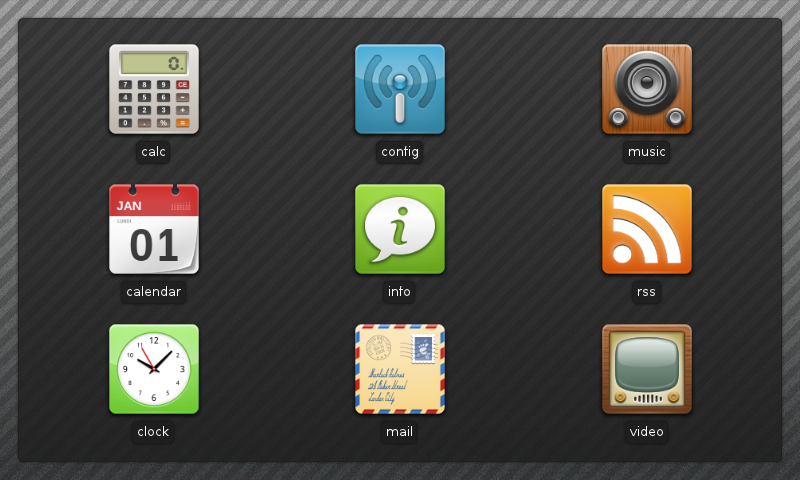
\includegraphics[scale=0.5]{images/screenshot1.png}
  \end{center}
  \caption{Interface edje à la fin de ce tutoriel}
\end{figure}

\section{Les Images}
\subsection{Les parts de type IMAGE}
Les explications de cette section portent sur le fichier
\href{file://tut02/tut02.edc}{tut02/tut02.edc}.

En partant du premier exemple, nous allons ajouter un fichier qui sera le fond
de notre interface.

Edje supporte un large type d'images, celles supportées par Evas,
PNG, JPEG, TIFF, BMP, ...
Pour décrire une image, il faut créer un ``part'' de type ``IMAGE'',
et dire à Edje quelle image insérer :

\begin{lstlisting}
 part {
   name: "Fond";
   type: IMAGE;
   description {
     state: "default" 0.0;
     image.normal: "bg.jpg";
   }
 }
\end{lstlisting}
\subsection{La directive images}
Comme nous avons vu précédemment, le fichier EDJ généré contient toutes les
ressources de notre interface, images incluses. Si nous compilons avec edje\_cc
ce fichier, ``bg.jpg'' ne sera pas trouvé dans nos ressources. Il faut ajouter
cette image dans la collection. Ceci est réalisé par l'ajout de cette directive
:
\begin{lstlisting}
   images {
      image: "bg.jpg" COMP;
   }
\end{lstlisting}

A quoi correspond ``COMP'' ? Edje ajoute les images dans le fichier binaire EDJ,
et nous pouvons lui dire de compresser ou non cette image.
Plusieurs type de compressions sont supportés :
\begin{itemize}
\item RAW: sans compression.
\item COMP: compression sans perte, comparable au format PNG.
\item LOSSY [0-100]: compression avec perte avec une qualité pouvant aller
de 0 à 100, comparable au format JPEG
\item USER: l'image n'est pas intégrée au fichier edje, mais est lue depuis
le disque.
\end{itemize}

Attention cependant, si vous utilisez la balise RAW, à la taille
finale de votre fichier binaire.
Pour une image de 800x600 en 32bits de couleurs (RGBA), la taille embarquée dans
le fichier binaire sera : 800x600x4 ~= 1.8MO !

\subsection{edje\_cc et les images}
Le compilateur edje cherche les images dans les répertoires relativement au
répertoire où il est executé.
Nous avons la possibilité de donner l'emplacement relative dans nos fichiers
EDC. Par exemple :

\begin{lstlisting}
   images {
      image: "images\bg.jpg" COMP;
   }
\end{lstlisting}

Ceci peut très vite devenir rébarbatif et long à écrire, nous pouvons donc
ajouter les répertoires qui contiennent nos images en utilisant l'argument
``-id'' (image directory) de edje\_cc

\begin{lstlisting}
edje_cc -id images -id images\icons file.edc
\end{lstlisting}

Pour faciliter la compilation, vous trouverez dans le répertoire de ce tutorial,
un script shell qui permet de compiler tous les fichiers EDC (et C dans la
suite) nommé build.sh

\begin{lstlisting}
.\build.sh #compile l'intégralité des exemples.
.\build.sh #tut02 compile l'exemple contenu dans le repertoire tut02
\end{lstlisting}

Les fichiers binaires sont quant à eux générés dans le répertoire build.

\subsection{Les motifs}
Edje permet également l'affichage de motifs à l'écran en répétant une images.
Le fichier \href{file://tut03/tut03.edc}{tut03/tut03.edc} montre comment
utiliser une image motif avec la balise fill
\begin{lstlisting}
 size {
   relative: 0.0 0.0;
   offset: 20 20;
 }
\end{lstlisting}

Dans notre cas l'image a une taille de 20x20px nous voulons qu'elle soit répétée
sur l'axe des X et des Y.

Il y a plusieurs autres options permettant de répéter les motifs, je vous laisse
les découvrir par vous même, tout est décrit dans la
\href{http://docs.enlightenment.org/auto/edje/edcref.html}[documentation de edje]


\section{Le Texte}

\subsection{Description d'une icône}
Regardons le code du fichier \href{file://tut04/tut04.edc}{tut04/tut04.edc} plus
en détail. Un nouveau groupe a été ajouté, nommée ``icon''. Il contient une
image ``icon.png'' et un nouveau part de type ``TEXT''.

\begin{lstlisting}
  part {
    name: "text";
    type: TEXT;
    description {
      state: "default" 0.0;
      color: 0 0 0 255;
      text {
        font: "Sans";
        size: 12;
        text: "Description";
      }
    }
  }
\end{lstlisting}

Les différentes options parlent d'elle même :
\begin{itemize}
\item Couleur du texte : Noir;
\item Fonte utilisée ``Sans'';
\item Taille de la fonte : 12;
\item Texte à afficher ``Description'';
\end{itemize}

Regardons à quoi ressemble notre exemple avec edje\_player. Attention dans cet
exemple nous avons deux groupes. Nous devons donc spécifier à ejde\_player quel
groupe nous voulons visualiser, et nous allons également lui dire de changer la
couleur de fond.

\begin{lstlisting}
edje_player -c=255,255,255,255 -g icon tut04.edj
\end{lstlisting}

Nous sommes loin du résultat escompté ! Par défaut tous les ``parts'' sont
centrés au centre de l'écran et occupent toute la taille du groupe. Nous devons
décrire comment les objets sont placés les uns par rapport aux autres.
C'est l'objet des tutoriels 5 à 8.


\section{Placement des objets}
\subsection{Proportions}

L'icône se doit d'être carrée, c'est le cas de toutes les icônes en informatique
non ?  Pour cela Edje propose la balise ``aspect'' et ``aspect\_preference''. Ces deux
balises sont liées. Regardons à quoi ça ressemble pour un définir un ``part'' carré:
\begin{lstlisting}
  aspect: 1.0 1.0;
  aspect_preference: BOTH;
\end{lstlisting}

``aspect'' prend deux flottants comme paramètres, min et max. Dans un cas normal,
les dimensions de l'objet ne sont pas liées, en utilisant le paramètre ``aspect'',
on force Edje à garder un ratio entre la largeur et la hauteur de notre ``part''.
Dans le cas 1.0 1.0 l'icône aura donc même hauteur et largeur.
``aspect\_preference'' lui donne la direction dans laquelle on veut que ce ration s'applique.
Rien de mieux pour comprendre qu'un exemple. Regardez les fichiers tut05.1.edj,
tut05.2.edj et tut05.3.edj pour visualiser les effets de ``aspect'' et
``aspect\_preference''.

\subsection{Positions relative et absolue}

Edje permet de positionner les objets les uns par rapport aux autres de deux
façons. Positionnement relatif et positionnement absolu.

Le positionnement relatif est en pourcent, 1.0 représente 100\% et 0.0 0\%. Vous
pouvez également spécifier des valeurs supérieures à 1.0 et inférieures à 0.0,
dans le cas ou vous voulez que votre part s'affiche au dela du part parent,
alors que les positions absolues sont en pixels.

Les balises ``rel1'' et ``rel2'' permettent de donner la position d'un objet par rapport
à un autre. Par défaut la position est celle par rapport au groupe.
Le positionnement relatif est donné avec la balise ``rel1.relative'' et
``rel2.relative'' alors que le positionnement absolu est donnée par ``rel1.offset'' et
``rel2.offset''.

\begin{figure}
  \begin{center}
    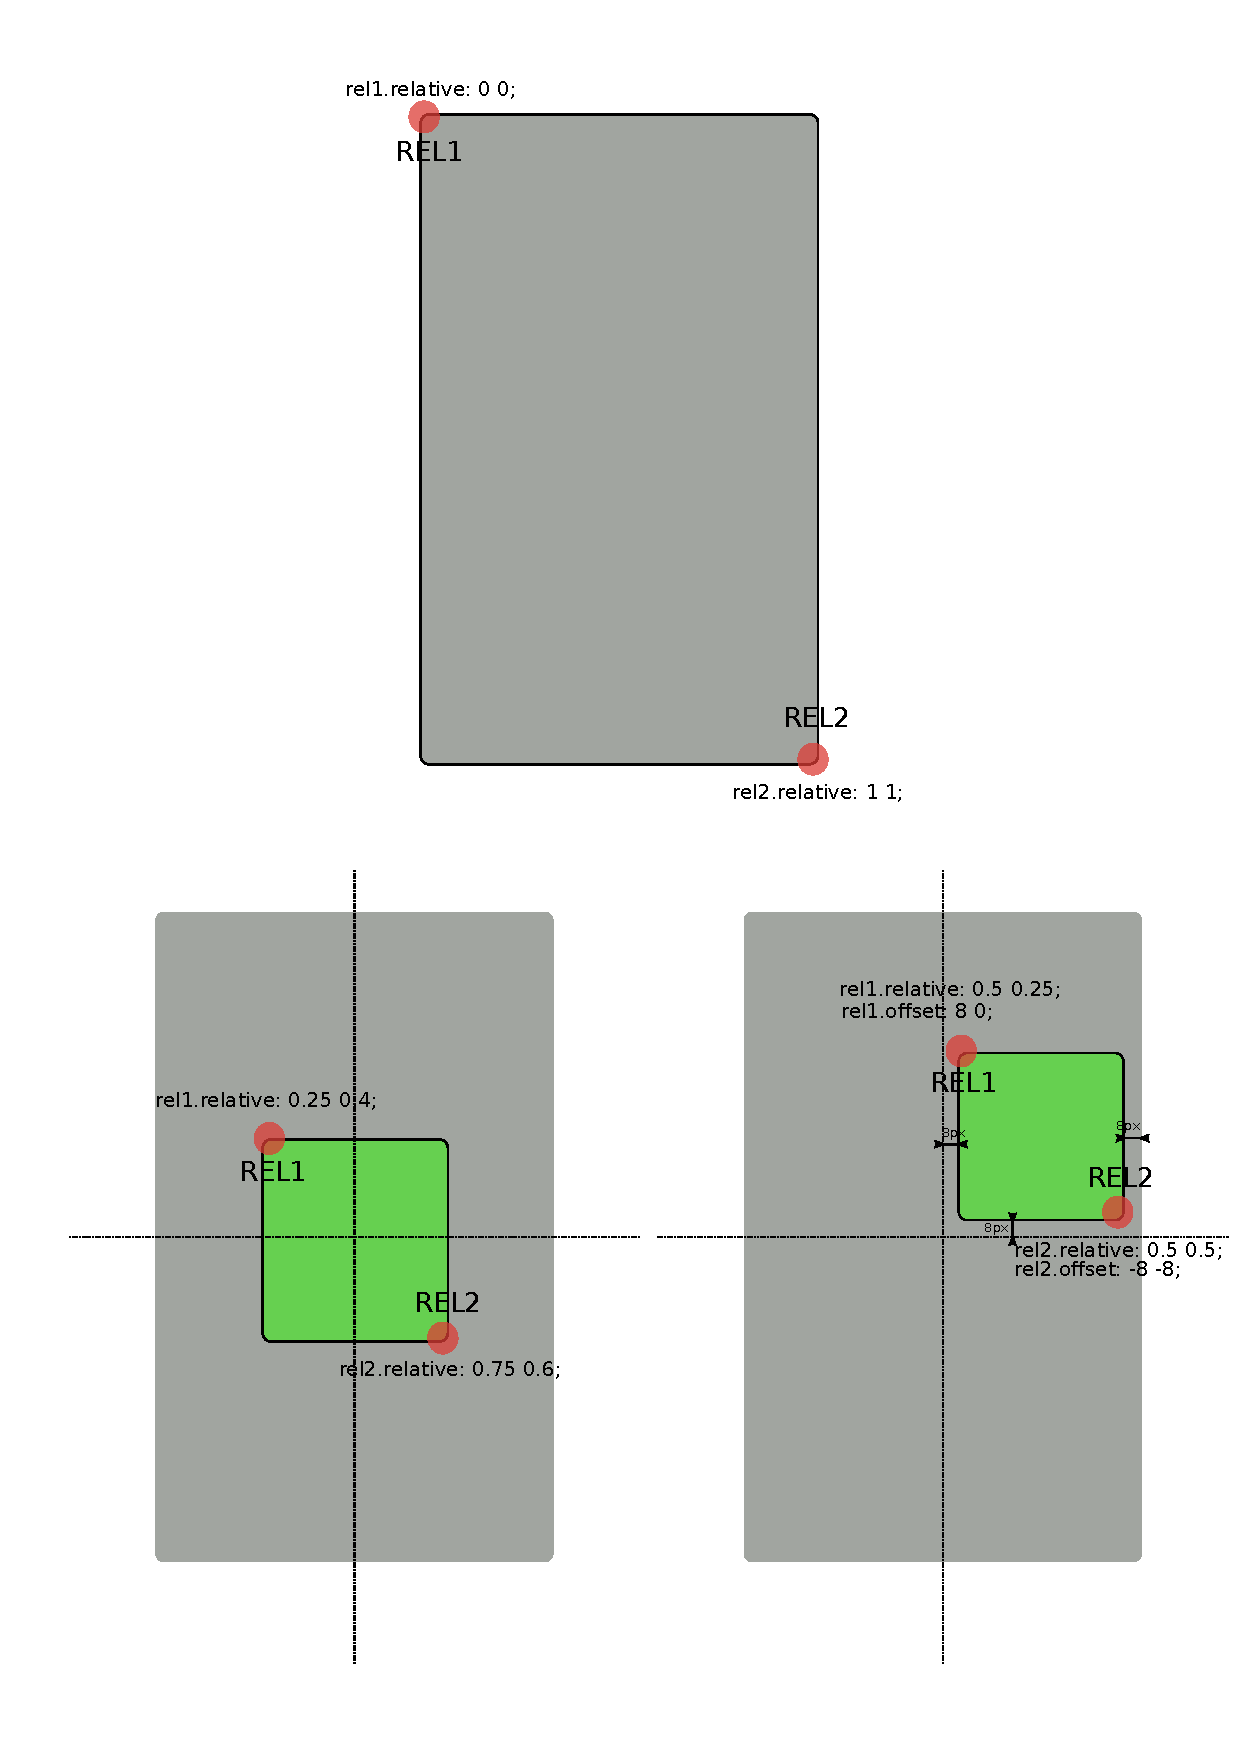
\includegraphics[scale=0.7]{images/rel1rel2.pdf}
  \end{center}
  \caption{Positionnement relatif et absolu}
\end{figure}

Dans cet exemple le positionnement est relatif au groupe, mais nous pouvons
spécifier un positionnement par rapport à un autre ``part'' en utilisant la balise :

\begin{lstlisting}
rel1.to: "autre_part1";
rel1.to: "autre_part2";
\end{lstlisting}

Ou encore relativement à un autre ``part'' mais uniquement sur un des axes X ou Y :
\begin{lstlisting}
rel1.to_x: "autre_part1";
rel1.to_y: "autre_part2";
\end{lstlisting}


Pour l'exemple du fichier tut06.edc, j'ai choisi de positionner le texte en bas
du groupe. Le texte pouvant être dynamique, comme nous allons voir plus loin,
nous pouvons demander à Edje de calculer sa taille, c'est le rôle de
\begin{lstlisting}
min: 1 1;
\end{lstlisting}

Edje va calculer la hauteur et la largeur du texte en fonction de la police,
et le ``part'' aura donc cette taille. Il nous reste plus qu'ensuite à positionner
l'icône au dessus de ce texte (balise rel2.to: \"texte\")
On ajoute également un bord de 8 pixels autour de l'icône pour plus de
lisibilité.
\begin{lstlisting}
  rel1.relative: 0 0;
  rel1.offset: 8 8;
  rel2.relative: 1 0;
  rel2.offset: -7 -7;
  rel2.to: "text";
\end{lstlisting}

Vous verrez également une telle description sous cette forme :
\begin{lstlisting}
  rel1 {
    relative: 0 0;
    offset: 8 8;
  }
  rel2 {
    relative: 1 0;
    offset: -7 -7;
    to: "text";
  }
\end{lstlisting}

Ces deux notations sont équivalentes.

\section{Images bordurées}

Nous arrivons ici à une des fonctionnalités que je préfère dans Edje ! Les
bords (borders en anglais). Ça tient en une ligne, mais ça rend de grands
services.

\begin{lstlisting}
image.border: 8 8 8 8;
\end{lstlisting}

C'est spécifique aux ``parts'' de type ``IMAGES''. Cette ligne impose à Edje de ne
redimensionner toutes les parties de l'image, sauf les bordures. Le cas se
présente lorsque on utilise une image avec des coins arrondis par
exemple, comme c'est le cas avec le contour du texte.

Les paramètres de cette balise sont les suivants : left, right, top, width et les
paramètres sont donnés en pixels.

\begin{figure}
  \begin{center}
    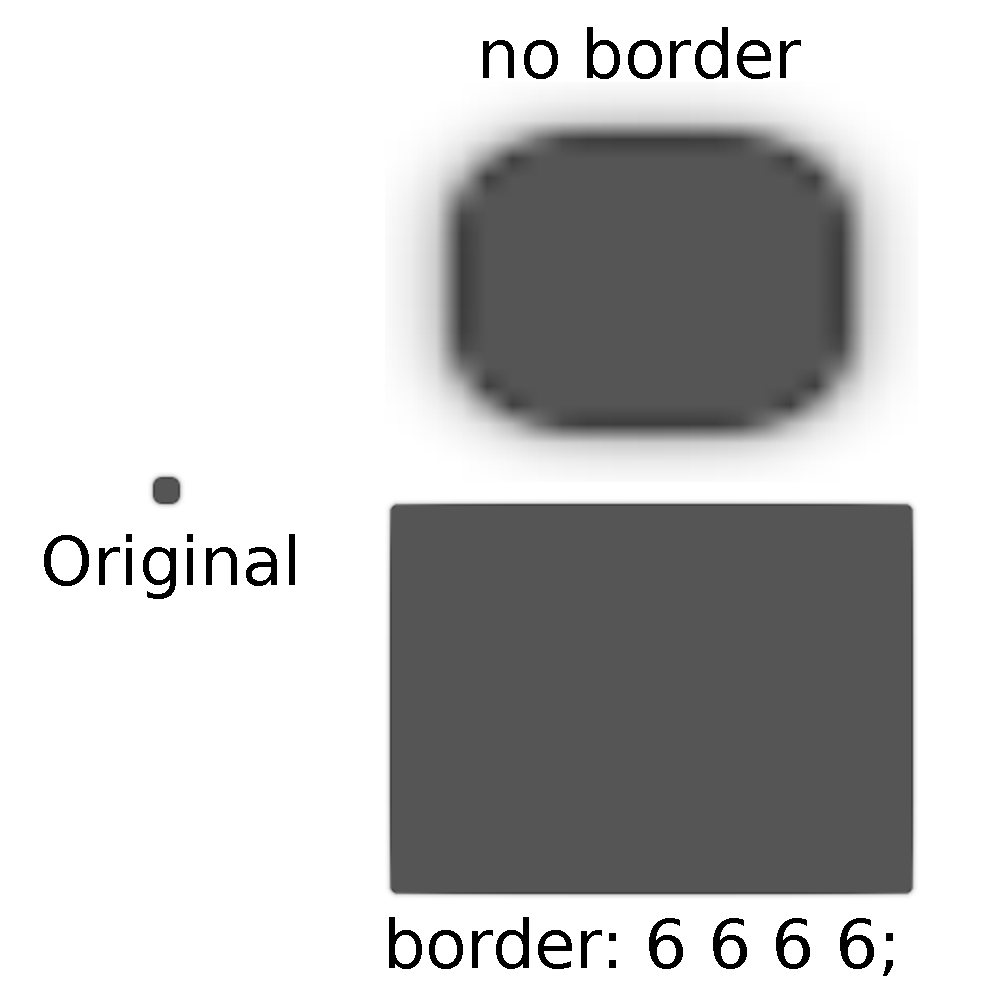
\includegraphics[scale=0.5]{images/border_diff.pdf}
  \end{center}
  \caption{Avec et sans bord}
\end{figure}


\begin{figure}
  \begin{center}
    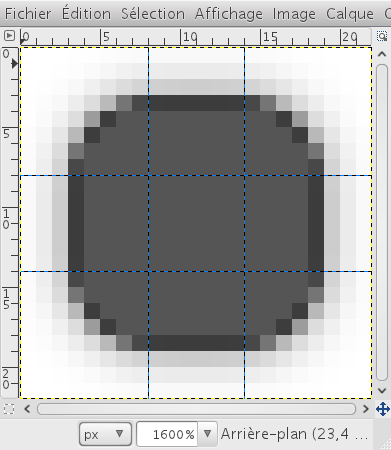
\includegraphics[scale=0.5]{images/border2.png}
  \end{center}
  \caption{Gimp et bords}
\end{figure}



\section{Les programmes}

\subsection{Evènements souris}

Pour nous simplifier la vie par la suite, j'ai ajouté dans le fichier tut09
un ``part'' que j'ai nommé ``events'', qui se place au dessus de tous les autres
``parts''. L'ordre des ``parts'' est fonction de la position de la description dans le
groupe. C'est-à-dire que le ``part'' le plus bas dans le fichier est le plus haut
dans l'interface.

Ce ``part'' ``events'' semble ne servir à rien, puisqu'il a une transparence à 0,
mais il va nous rendre de grands services. Dans la suite il va nous permettre de
capturer tous les évènements souris de notre icône.

La balise ``visible'' indique à Edje si le ``part'' doit être affiché ou pas à l'écran
quelque soit la position, la taille ou toute autre propriété du ``part''.
Par défaut les ``parts'' sont visibles, mais parfois, nous pouvons faire en sorte
qu'un ``part'' devienne invisible. Nous voudrions par exemple à moment donné que
les évènements souris ne soient pas capturés, Il nous suffirait dont de mettre
cette propriété à 0 pour que plus aucun évènement ne soit traité pour ce
``part''.

\subsection{Les Programmes}

Un programme est une action que Edje va réaliser. Ils peuvent être de différents
types, un événement souris sur notre groupe, une signal provenant du programme
qui manipule notre groupe, un signal envoyé par un autre programme, un signal
envoyé par Edje.

Le fichier tut10.edc présente un exemple de programme qui réagit à un événement
bouton 1 de la souris enfoncé :

\begin{lstlisting}
  program {
    name: "mouse_down";
    signal: "mouse,down,1";
    source: "events";
    action: STATE_SET "down" 0.0;
    target: "icon";
  }
\end{lstlisting}

Voilà à quoi correspondent les différentes balises :

\begin{itemize}
\item name: C'est le nom du programme
\item signal: c'est la chaîne de caractères qui définit le signal reçu, dans ce
cas c'est un signal envoyé par edje lorsque le bouton 1 de la souris est enfoncé
sur le ``part'' défini dans la balise ``source''.
\item source: le ``part'' qui est responsable du signal. Le bouton de la souris doit être enfoncé sur ce
``part''. On voit ici que ce ``part'' nous sert à quelque chose ! Si il n'existait pas
nous aurions dû dupliquer ce programme pour réaliser l'action sur le ``part'' icon,
texte et texte\_bg !
\item action: L'action à réalisr lorsque le signal est reçu. Ici nous demandons
à Edje de changer l'état du part défini dans la balise ``target'' à "down" 0.0
\end{itemize}

Un ``part'' peut avoir plusieurs états, si il existe plusieurs descriptions de celui-ci.
C'est le rôle de la balise ``description'' que nous avons rencontrée mais pas
encore expliquée.

Tous les paramètres d'un ``part'' que nous avons vu jusqu'à présent (couleur,
alignement, la fonte ou la taille pour un texte, ....) peuvent avoir différentes
valeurs d'une description à une autre.

\begin{lstlisting}
state: "default" 0.0;
\end{lstlisting}

Cette balise permet de donner un nom à notre état, ainsi qu'un flottant.
Revenons à notre exemple :

\begin{lstlisting}
  part {
    name: "icon";
    type: IMAGE;
    mouse_events: 0;
    description {
      state: "default" 0.0;
      aspect: 1.0 1.0;
      aspect_preference: BOTH;
      image.normal: "icon.png";
      rel1.relative: 0 0;
      rel1.offset: 8 8;
      rel2.relative: 1 0;
      rel2.offset: -7 -7;
      rel2.to_y: "text";
      align: 0.5 0.5;
    }
    description {
      state: "down" 0.0;
      inherit: "default" 0.0;
      color: 255 255 255 128;
    }
  }
\end{lstlisting}

Ici nous avons deux états : \"default\" 0.0 et \"down\" 0.0.
L'état down, hérite de toutes les propriétés de ``default'' sauf pour la couleur, où
nous changeons l'alpha.

Couplé au programme précédent, cela aura pour effet de changer la transparence
lors d'un clic sur l'icône.

Nous pouvons vérifier ceci avec edje\_player :
\begin{lstlisting}
edje\_player tut10.edj -g icon
\end{lstlisting}

Effectivement la couleur change, mais lorsque nous relâchons le clic, notre
icône reste dans cet état. Nous devons ajouter le programme équivalent pour le
``mouse up''. Le fichier tut11.edc montre ceci.

\subsection{Les animations}

Comme nous pouvons voir, la transition est abrupte. Pour réaliser un effet plus
relaxant, nous allons ajouter une animation entre deux états de nos ``parts''.

\begin{lstlisting}
  transition: LINEAR 1.0;
\end{lstlisting}

La balise transition permet, comme son nom l'indique, d'indiquer à Edje qu'il
doit changer l'état, et que ce changement doit durer 1 seconde.
Entre nos deux états Edje va interpoler la position et la couleur de notre
objet et cet interpolation sera de type linéaire. Le framerate par défaut de
Edje et de 60 images par secondes, il va donc calculer 60 images clés différentes
pour notre part.

\begin{figure}
  \begin{center}
    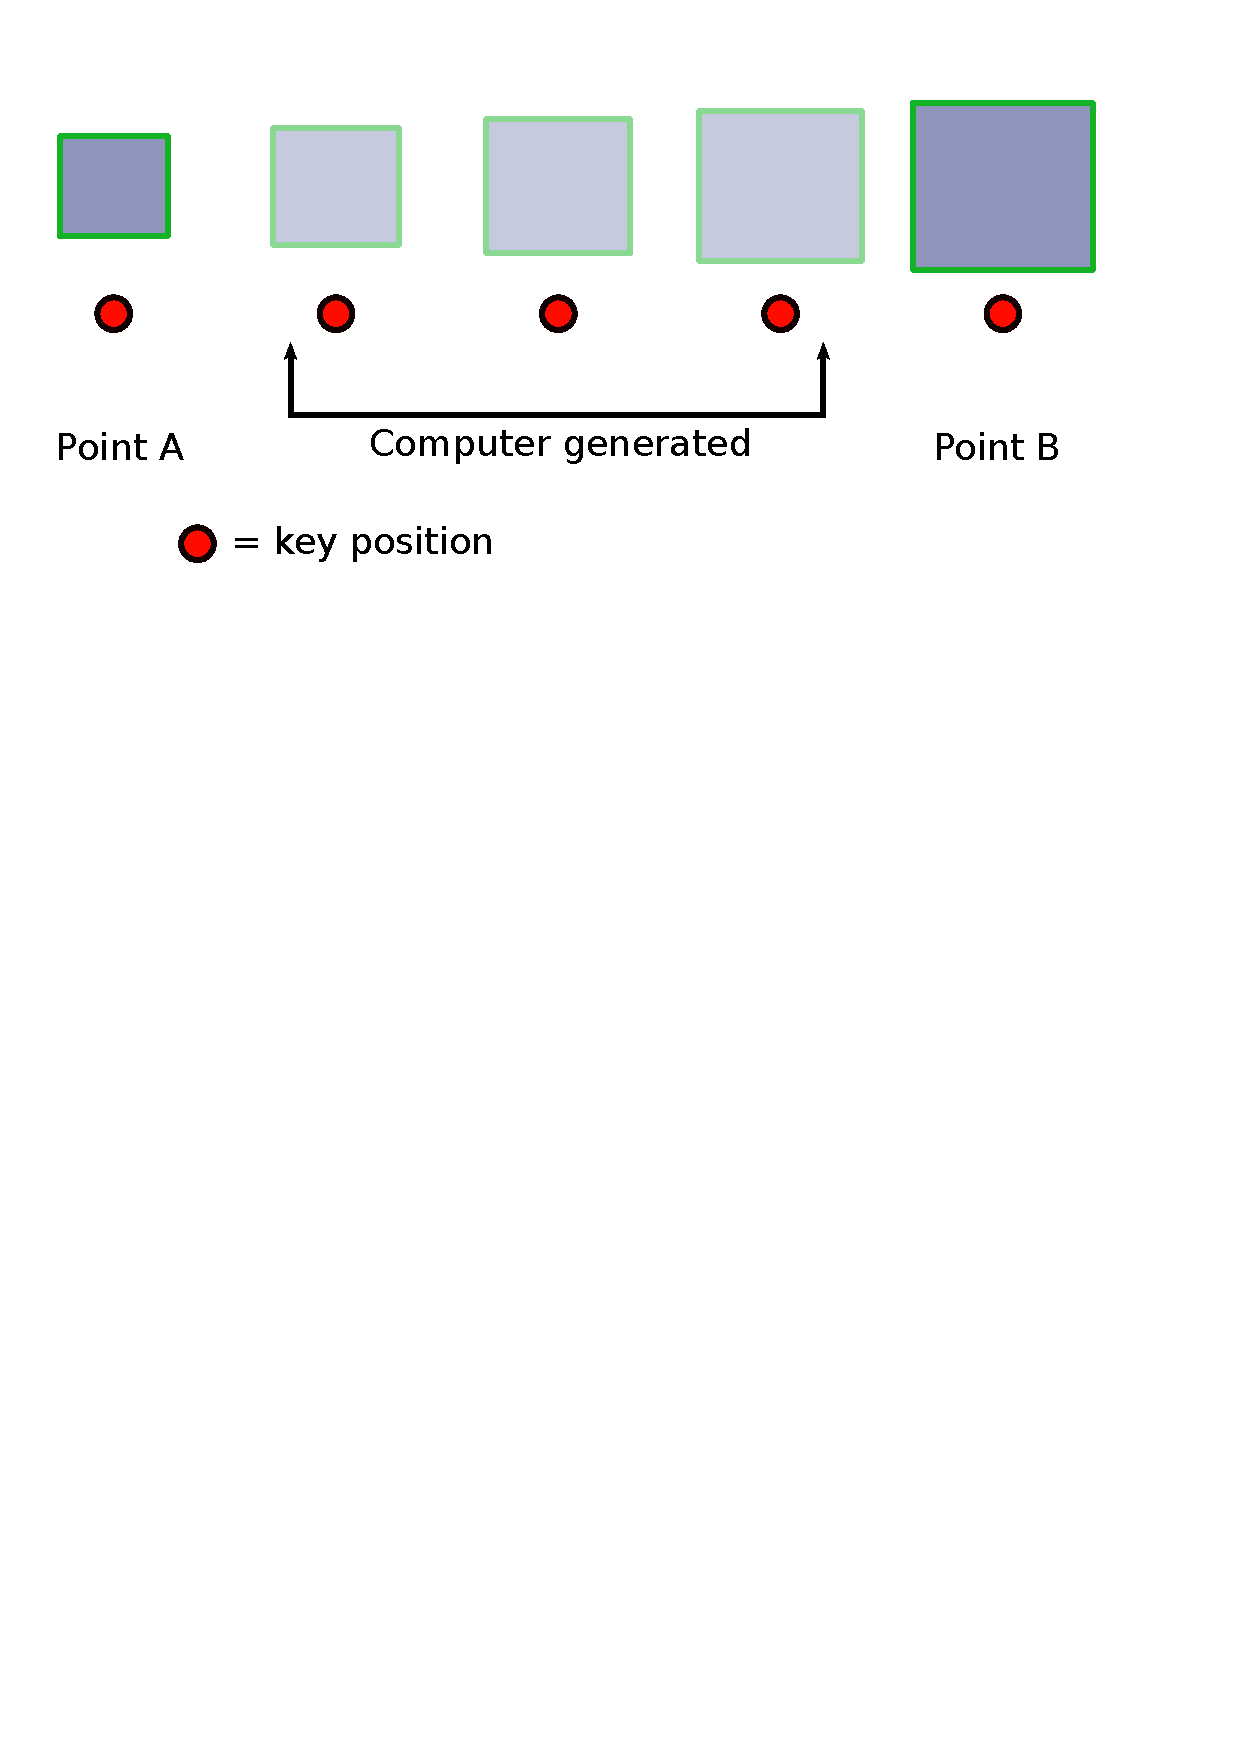
\includegraphics[scale=0.5]{images/animation.pdf}
  \end{center}
  \caption{Création des images clés}
\end{figure}

\section{Intégrer un objet Edje dans un programme C}
Nous avons décrit des objets, nous avons généré le binaire et nous avons testé
le tout avec edje\_player. Mais notre but est de créer un interface, donc créer un
exécutable.

Dans ce chapitre, nous allons voir comment intégrer les groupes que nous avons
créés dans une application Elementary.

Pourquoi avec Elementary et pas avec Edje ? Tout simplement parce que c'est plus
simple, et concis avec Elementary, que Elementary utilise Edje pour nous et que
je suis plutôt de nature fainéante !

Tout d'abord créons un programme très simple qui crée une fenêtre avec un titre,
et qui quitte lorsque on clique sur la croix. (fichier tut13.c)
\begin{lstlisting}
  /* gcc -o test tut13.c `pkg-config elementary --cflags --libs` */

  #include <Elementary.h>

  static void
  _win_del(void *data, Evas_Object *obj, void *event_info)
  {
    elm_exit();
  }

  int main(int argc, char **argv)
  {
    Evas_Object *win;

    elm_init(argc, argv);

    win = elm_win_add(NULL, "tuto", ELM_WIN_BASIC);
    elm_win_title_set(win, "Edje Tutorial");
    evas_object_smart_callback_add(win, "delete,request", _win_del, NULL);

    evas_object_resize(win, 800, 480);

    evas_object_show(win);

    elm_run();
    elm_shutdown();
  }
\end{lstlisting}

Maintenant ajoutons notre groupe ``interface'' que nous avons créé au tout
début de ce tutoriel dans notre fenêtre :

\begin{lstlisting}
  layout = elm_layout_add(win);
  elm_layout_file_set(layout, "tut14.edj", "interface");
  evas_object_show(layout);
\end{lstlisting}

Et faisons en sorte que celui-ci soit redimensionné lorsqu'on redimensionne la
fenêtre :
\begin{lstlisting}
   elm_win_resize_object_add(win, layout);
\end{lstlisting}

Nous rencontrons ici un des concepts les plus importants de Evas. Les Smart
Objects. elm\_layout\_add utilise Edje en interne, et crée un Smart Objet qui
pourra ensuite être manipulé par les primitives de Evas (move, resize, ....)
Nous demandons ensuite à ce que cet objet utilise le groupe \"interface\# du
fichier tut14.edj. Et nous affichons cet objet à l'écran avec
evas\_object\_show. elm\_win\_resize\_object\_add va faire en sorte que Evas
redimensionne notre objet à la taille de la fenêtre.

Recompilons notre programme et testons :
\begin{lstlisting}
./tut14
\end{lstlisting}

Nous avons écrit notre premier programme intégrant un objet edje !

Rajoutons maintenant le groupe icon : (fichier tut15.c)
\begin{lstlisting}
   icon = elm_layout_add(win);
   elm_layout_file_set(icon, "tut14.edj", "icon");
   evas_object_resize(icon, 256, 256);
   evas_object_move(icon, 64, 64);
   evas_object_show(icon);
\end{lstlisting}

Notre Smart Object est créé comme précédemment, et cette fois-ci nous allons
le manipuler nous même, en lui donnant une taille de 256x256px et en le
plaçant en haut à gauche x=64px et y=64px.

Notre icône possède un texte (part \"text\", que nous allons changer grâce à :
\begin{lstlisting}
   elm_layout_text_set(icon, "text", "Vers l'infini et au delà!");
\end{lstlisting}

Elementary my dear Watson !

\subsection{La multiplication des icônes}
Notre exemple final contient plus qu'une seule icône. Machinalement, nous
pourrions dupliquer à la fois dans Edje et dans le code C les blocs permettant
de changer le nom de l'icône et le texte. Mais cela serait d'une part très long,
d'autre part source d'erreur mais surtout très rébarbatif. Et comme je le disais précédemment
je suis fainéant. Nous allons donc utiliser ce que Edje nous propose pour nous
faciliter la vie.

Les descriptions Edje sont préprocéssées. Comme les fichier .c et .h par le
programme cpp. Le rôle de celui-ci est de remplacer les toute occurrence d'une
macro dans le texte par le morceau de code défini dans la macro. Lorsqu'il
rencontre un \#include il copie l'intégralité de ce fichier à cette position.

Comme dans un programme C, nous allons donc créer une macro ICON pour nous
faciliter la vie.

Notre macro prendra comme paramètre d'entrée le nom de l'icône et le nom du
fichier icône à utiliser.

Nous pouvons ensuite ajouter nos différents groupes comme ceci :
\begin{lstlisting}
   ICON("video.png", "video");
   ICON("meteo.png", "meteo");
   ICON("calc.png", "calc");
   ICON("music.png", "music");
   ICON("calendar.png", "calendar");
   ICON("mail.png", "mail");
   ICON("rss.png", "rss");
\end{lstlisting}

\section{les tables}

Maintenant que nos groupes ont été ajoutés à notre fichier Edje, nous pourrions
afficher chaque icône à l'écran, les positionner les unes par rapport aux
autres avec evas\_object\_move. Cela serait fastidieux. D'autre part si nous
voulons changer le layout, il faudrait fournir une nouvelle version du programme
et l'avantage de Edje c'est de pouvoir faire ça pour nous.

Nous allons donc utiliser un nouveau type de parts, après les TEXT, les RECT et
les IMAGES : les TABLE.
Voici comment positionner les icônes que nous avons créées précédemment :
\begin{lstlisting}
  part {
    name: "table_description";
    type: TABLE;
    description {
      state: "default" 0.0;
      fixed: 1 1;
    }
    table {
      items {
        item {
          type: GROUP;
          source: "video";
          align: -1 -1;
          position: 0 0;
        }
        item {
          type: GROUP;
          source: "meteo";
          align: -1 -1;
          position: 0 1;
        }
        item {
          type: GROUP;
          source: "calc";
          position: 0 2;
          align: -1 -1;
        }
        item {
          type: GROUP;
          source: "music";
          position: 1 0;
          align: -1 -1;
        }
        item {
          type: GROUP;
          source: "calendar";
          position: 1 1;
          align: -1 -1;
        }
        item {
          type: GROUP;
          source: "mail";
          position: 1 2;
          align: -1 -1;
        }
        item {
          type: GROUP;
          source: "rss";
          position: 2 0;
          align: -1 -1;
        }
      }
    }
  }
\end{lstlisting}

Chaque ``item'' de la table a une balise position, qui donne sa positon dans la
table. La petite subtilité ici est l'alignement de chaque ``item''. On demande
à Edje de désactiver l'alignement (valeur -1) et donc de s'adapter à la taille
de la cellule.

\section{Icônes et multi-résolution}

Nous allons étudier ici une autre fonctionnalité intéressante de Edje, les ``set
d'icônes''. Nous voulons que notre application s'affiche quelque soit sa taille
et nous somme aidés par l'utilisation de la balise ``border'' dans les images.
Imaginons que nous voulons intégrer des icônes qui s'affichent aussi bien en
512x512 que en 16x16. Nous avons plusieurs possibilités.
La plus simple est d'utiliser une icône source de 512x512. Dans le cas d'un
affichage en 16x16, celle-ci est réduite par Evas et Edje avec la perte
d'informations que cela amène. Une autre solution serait d'utiliser une image
de type SVG, qui s'adaptera en fonction de la résolution. Mais le plus souvent
ce type de fichier est très lourd à gérer, en tout cas bien plus qu'un fichier
bitmap.
Pour résoudre ce problème, Edje intègre les set d'icônes. Nous pouvons lui
indiquer quelle image utiliser en fonction de la taille. Un autre type
d'utilisation de cette fonctionnalité et d'afficher une image complètement
différente en fonction de la taille de la zone d'affichage.

Le fichier tut18 présente cette fonctionnalité. J'ai ajouté un script dans le
répertoire images, qui permet à partir d'un fichier svg source de générer les
fichiers png dans les différentes résolutions voulues.

Lorsque nous testons avec edje\_player -g calc tut18.edj, et que nous
redimensionnons la fenêtre, on peut voir que Edje adapte la résolution de
l'icône à la taille.

\section{Les Containeurs}

Nous avons vu comment créer des groupes, et comment ajouter ces groupes via
notre programme.
Dans le cas du fond d'écran, c'est un layout Evas qui affiche un Objet Edje.
Dans le cas de l'icône, c'est un layout Edje avec pilotage Edje, puisque c'est
la table qui fait l'affichage et le layout.
La fonctionnalité que nous allons voir, c'est la troisième possibilité :
un layout Edje avec pilotage par Evas : les Swallows ou conteneurs.
C'est un ``part'' de type SWALLOW. C'est une zone, qui comme les autres ``parts'' peut
avoir différentes positions, tailles, .... en fonction de la description et qui
peut contenir un Smart Object. C'est notre programme qui décidera quoi mettre
à l'intérieur.

Voici un exemple de part de type swallow :
\begin{lstlisting}
  part {
    name: "table_swallow";
    type: SWALLOW;
    description {
      state: "default" 0.0;
      rel1.to: "table_bg";
      rel2.to: "table_bg";
    }
  }
\end{lstlisting}

et côté programme, on crée un rectangle avec Evas et on l'ajoute dans notre part
\begin{lstlisting}
   rect = evas_object_rectangle_add(evas_object_evas_get(win));
   evas_object_color_set(rect, 0, 255, 0, 128);
   evas_object_resize(rect, 10000, 10000);
   evas_object_move(rect, -5000, -5000);
   evas_object_show(rect);
   elm_layout_content_set(layout, "table_swallow", rect);
\end{lstlisting}

Comme on peut le voir ici, j'ai changé la position de l'objet ainsi que sa
taille en donnant des valeurs absurdes, on voit bien en exécutant tut19 que
Edje gère l'affichage de notre objet.

Nous avons ajouté un rectangle mais nous pouvons ajouter n'importe quel type
de Smart Objects.
Dans l'exemple suivant, nous allons ajouter un panel à notre interface, qui
affichera sous forme de texte des infos à l'écran. Et lorsque nous cliquerons
sur l'icône info, nous afficherons ce nouveau groupe à l'écran depuis notre
programme.

\section{les TEXTBLOCKS}

Notre panneau d'information affichera du texte. Tout à l'heure nous avons
ajouté un nom à notre icône. Mais celui-ci avait une couleur unique. Si nous
voulons ajouter des styles de texte différents, afficher le texte sur plusieurs
ligne, Edje propose pour cela les TEXTBLOCKS.

Edje utilise un système de marqueurs pour différencier les différents styles.
Si vous connaissez les balises html, vous ne serez pas perdu ici.
Un style ressemble à ceci :
\begin{lstlisting}
  styles {
    style { name: "textblock_style";
      base: "font=Sans font_size=16 color=#EEE wrap=word";
      tag:  "br" "\n";
      tag:  "ps" "ps";
      tag:  "hilight" "+ font=Sans:style=Bold color=#3dadff";
      tag:  "b" "+ font=Sans:style=Bold colo=#2d3e46";
      tag:  "tab" "\t";
      tag:  "h1" "+ font_size=40 color=#b5de29";
      tag:  "h2" "+ font_size=30";
      tag:  "h3" "+ font_size=30";
      tag:  "h4" "+ font_size=18";
      tag:  "rhinoceros" "+ color=#F0F";
      tag:  "link" "+ color=#00000080";
    }
  }
\end{lstlisting}

Comme toujours un nom, unique, auquel on pourra faire référence.
Une base, qui est la valeur par défaut de notre texte, c'est-à-dire
quand nous n'utilisons pas de balise. Et enfin les tags, qui définissent
chacune des balises que nous pouvons utiliser pour ce style.
J'ai défini des balises que nous retrouvons pour la plus part dans le HTML.
Mais nous pouvons mettre dans le nom des tags ce que nous voulons.
C'est le cas par exemple de la balise ``rhinocéros''. Elle change uniquement
la couleur du texte, mais comme on peut le voir pour les autres balises, on peut
changer la fonte du texte, sa couleur, sa taille.....

Une fois un style défini, nous pouvons déclarer notre nouveau part de type
TEXTBLOCK :

\begin{lstlisting}
  part {
    name: "textblock";
    type: TEXTBLOCK;
    entry_mode: EDITABLE;
    source5: "anchor";
    description {
      state: "default" 0.0;

      text {
        style: "textblock_style";
      }
    }
  }
\end{lstlisting}

Dans notre programme nous pouvons spécifier le texte comme tout à l'heure, mais
aussi enrober certaines parties avec les balises que nous avons définies dans le style.

\begin{lstlisting}
 elm_layout_text_set(textblock,"textblock", "<h1>What is Enlightenment?</h1><br>");
\end{lstlisting}

\section{Capturer les signaux edje dans le programme}

Pour avoir une interaction entre Edje et notre programme, nous pouvons utiliser
des programmes contenant l'action SIGNAL\_EMIT. Lorsque ce programme est
exécuté, Edje envoie alors ce signal. A nous de le capter et de réagir en
conséquence.
Voici le code d'exemple qui permet de capturer absolument tous les signaux émis
par le groupe ``layout'' :
\begin{lstlisting}
  edje = elm_layout_edje_get(table);
  edje_object_signal_callback_add(edje, "*", "*", _edje_signal_cb, NULL);
\end{lstlisting}

et le code du callback executé lorsque un signal est reçu :
\begin{lstlisting}
static void
_edje_signal_cb(void *data, Evas_Object *obj, const char *emission, const char *source)
{
   printf("Emission : %s - Source : %s\n", emission, source);
}
\end{lstlisting}

Les * utilisés dans l'ajout du callback permettent de filtrer les signaux, ici
nous affichons tout.

Pour le besoin de notre exemple, nous allons envoyer, lors d'un clic sur une
icône, le nom de l'icône.
\begin{lstlisting}
   program {                                                      \
     name: "mouse_click";
     signal: "mouse,clicked,1";
     source: "events";
     action: SIGNAL_EMIT "info,clicked" "";
   }
\end{lstlisting}

Attention ici, nous utilisons le signal ``mouse,clicked'', qui est différent de
``mouse down'' et ``mouse up''. Celui-ci est envoyé uniquement si on relâche la souris
au dessus de la source.

Dans le programme nous allons recevoir les données : emission == "info\_clicked"
et source == "".

Lorsque ``info\_clicked'' sera reçu, nous allons alors créer notre paneau, et
l'afficher à la place de la table.

\subsection{Les Ancres(anchors)}

Les textblock peuvent en plus du texte de différents styles être clickables.
C'est le rôle des ancres ..... blablablalbla

\subsection{Transformations 3D}

blablablalbalbalbal....

\end{document}

